\chapter{Literature Review} \label{lit_chap}
The Parareal algorithm is not the first attempt to parallelize the solution of time-dependent differential equation in temporal direction, since Nievergelt already in 1964 proposed a procedure in \cite{nievergelt1964parallel} that eventually led to the so called multiple shooting methods. In \cite{gander2007superlinear} the authors relate the Parareal algorithm to the multiple shooting methods, and also explains why Parareal can be thought of as a multigrid method. A historic overview of the development of parallel in time algorithms can be found in \cite{gander201550}. Here the author also present different strategies for parallelizing time-dependent differential equations. One such strategy are the already mentioned multiple shooting methods \cite{nievergelt1964parallel, bellen1989parallel}, which also include the Parareal algorithm. What characterizes such methods is that they only decompose the time domain. This separates the multiple shooting methods from waveform relaxation methods\cite{lelarasmee1982waveform,gander1996overlapping}, where the spatial domain is decomposed through time. The difference in these decomposition techniques is illustrated in figure \ref{fig:fig}. Other strategies presented are multigrid \cite{hackbusch1985parabolic,lubich1987multi,horton1995space} methods and direct solvers in space-time\cite{miranker1967parallel,maday2008parallelization,guttel2013parallel}.
\\
\begin{figure}[h]
\centering
\begin{subfigure}{.5\textwidth}
  \centering
  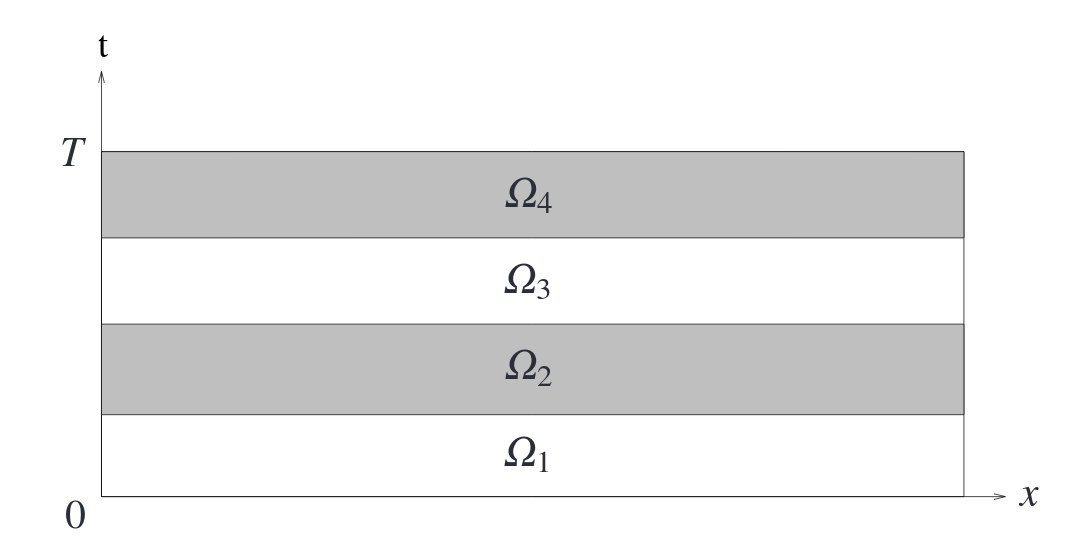
\includegraphics[width=.8\linewidth]{MSM.png}
  \caption{Multiple shooting decomposition}
  \label{fig:sfig1}
\end{subfigure}%
\begin{subfigure}{.5\textwidth}
  \centering
  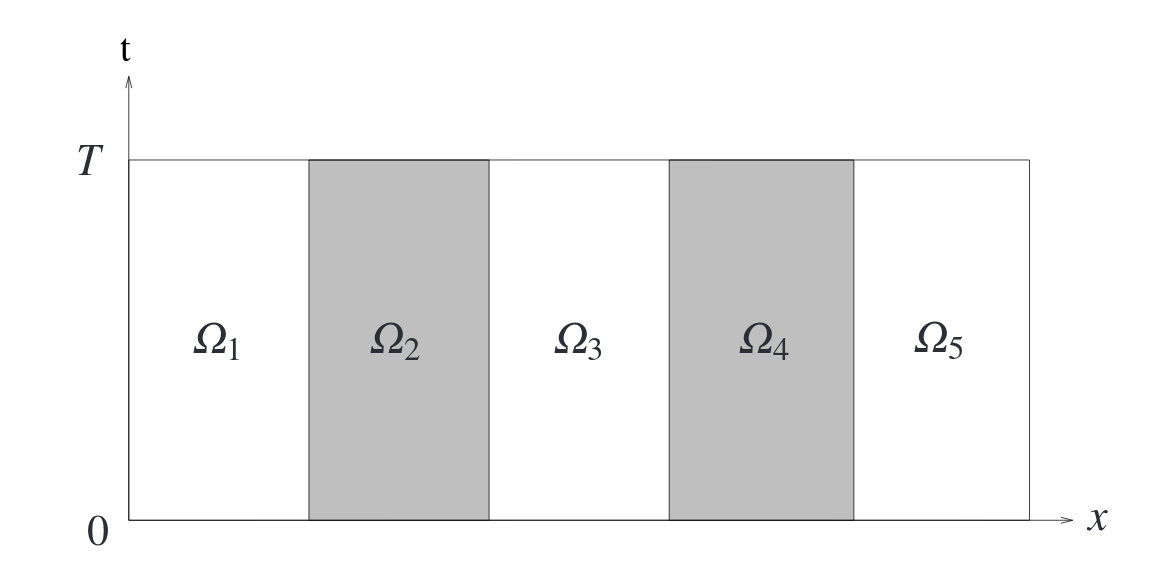
\includegraphics[width=.8\linewidth]{DDMinST.png}
  \caption{Waveform relaxation decomposition}
  \label{fig:sfig2}
\end{subfigure}
\caption{Different decomposition techniques for parallel in time algorithms. (a) shows the strictly temporal decomposition of multiple shooting methods. In (b) the decomposition is done spatially through time. Image source: \cite{gander201550}.}
\label{fig:fig}
\end{figure}
\noindent
\\
The Parareal algorithm was introduced by Lions, Maday and Turinici in \cite{lions2001resolution} as a way to solve differential evolution equations $f(y(t),t)=0$ with solution $y(t)$ in parallel. The idea is to combine a coarse (but fast) and fine (but slow) numerical scheme for discretization in time. To introduce parallelism we first decompose the time domain $I=[0,T]$ into $N$ subintervals $I_i=[T_{i-1},T_i]$. This gives us $N$ equations $f_i(y_i(t),t)=0$ defined on each interval $I_i$. 
\\
\\
The first step of the Parareal algorithm is to solve $f(y(t),t)=0$ sequentially on the entire interval using the coarse scheme. This gives us a (coarse) solution $Y(t)$ defined on the entire interval. We can then use $\{\lambda_i^0=Y(T_i)\}_{i=1}^{N-1}$ as initial conditions for the decomposed equations $f_{i+1}(y_{i+1}^0(t),t)=0$. The second step is then to solve these equations in parallel using the fine scheme, which will result in one solution $y_i(t)$ on each interval $I_i$. The idea then, is to utilize the difference $S_i^0=y_i^0(T_{i})-\lambda_i^0$ between coarse and fine solution to repeat this process in an iteration. This is done by propagating the differences $S_i^0$ with the coarse solver, to update the initial conditions for each decomposed equation. These new initial conditions $\lambda_i^1$ can then be used to solve the decomposed equations $f_{i+1}(y_{i+1}^1(t),t)=0$ in parallel with the fine solver. We can then define updated differences $S_i^1=y_i^1(T_{i})-\lambda_i^1$ and repeat the iteration until we are satisfied with the solution. A schematic presentation of the above described procedure can be viewed in figure \ref{trajectory_fig}. The version of Parareal presented in \cite{lions2001resolution} is most practical for use on linear equations. An alternative version of Parareal algorithm is found in \cite{baffico2002parallel}, which is equivalent to the one in \cite{lions2001resolution} for linear equations, but is easier applied to non-linear equations.
\\
\begin{figure}[h!]
\floatbox[{\capbeside\thisfloatsetup{capbesideposition={right,top},capbesidewidth=8cm}}]{figure}[\FBwidth]
{\caption{Schematic presentation of Parareal step. A first trajectory is generated using the coarse scehme (dashed line). Then starting from all points of this trajectory, we advance the equation with the fine scheme (arrow). The error is measured by $S^0_i=\Delta^0_i$. We generate the corrected trajectory (long dashed line) by propagating $S^0_i$ with the coarse scheme. This results in a trajectory closer to the exact trajectory (solid line). Notice that the Parareal trajectory is exact for the first time step. Source of image and caption:\cite{baffico2002parallel}.}\label{trajectory_fig}}
{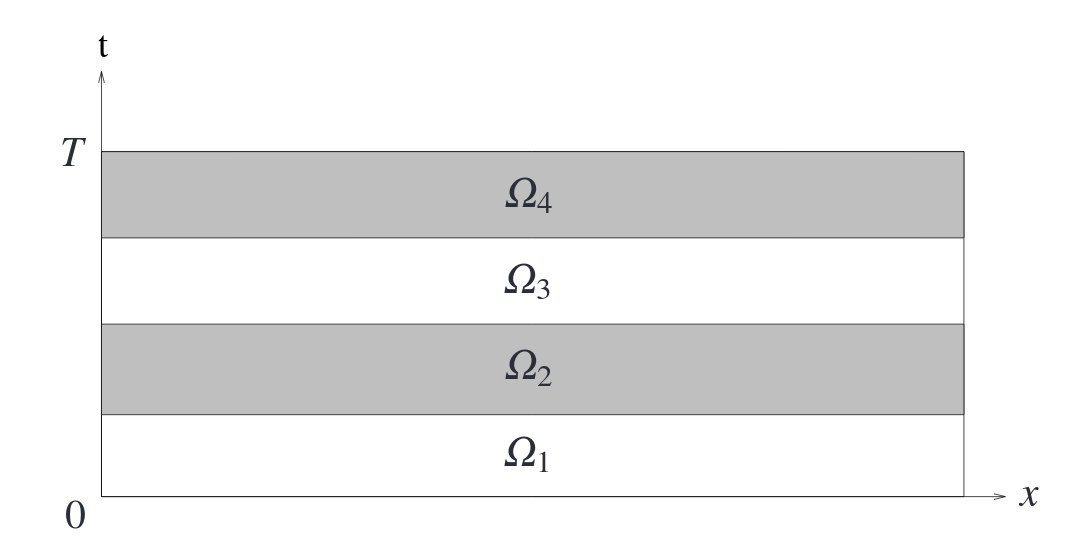
\includegraphics[width=5cm]{MSM.png}}
\end{figure}
\\
A lot of the work on the Parareal algorithm has been focused on establishing its stability and convergence properties. The stability results are found in \cite{staff2005stability},\cite{maday2007parareal} and \cite{bal2005convergence}. In \cite{staff2005stability,maday2007parareal} sufficient conditions for the stability of Parareal of autonomous differential equations (\ref{autonom E}) is derived:
\begin{align}
\frac{\partial y}{\partial t} =\rho y,\quad y(0)=y_0,\quad  \rho<0 \label{autonom E}
\end{align}
while \cite{bal2005convergence} presents more general stability results for parabolic equations. The stability of Parareal applied to hyperbolic equations is a more difficult question \cite{dai2013stable}. The convergence of Parareal is studied in \cite{lions2001resolution},\cite{bal2005convergence},\cite{gander2007analysis} and \cite{gander2007superlinear}. In \cite{lions2001resolution} Lions, Maday and Turinici show that $k$ iterations of the Parareal algorithm applied to equation (\ref{autonom E}) gives $\mathcal{O}(\Delta T^{k+1})$ order of accuracy if we use a coarse solver with order one accuracy and coarse time step $\Delta T$. This result is extended in \cite{bal2005convergence} to more general equations, and the order of accuracy is shown to be improved to $\mathcal{O}(\Delta T^{p(k+1)})$ when the coarse solver has order $p$. \cite{gander2007analysis,gander2007superlinear} return to analysis of equation (\ref{autonom E}). Instead of looking at a fixed number of iterations $k$, Gander and Vandewalle show convergence properties for the Parareal algorithm as the iteration count increases. They derived superlinear convergence for bounded time intervals and linear convergence for unbounded time intervals.
\\
\\
The Parareal algorithm has been applied to different equations, including on the Navier-Stokes equations\cite{fischer2005parareal}, to molecular-dynamics simulations\cite{baffico2002parallel}, to stochastic ordinary differential equations\cite{bal2003parallelization}, to reservoir simulations \cite{garrido2005convergent}, to fluid, structure and fluid-structure problems\cite{farhat2003time}, or on the American put\cite{bal2002parareal}. The success of applying the Parareal algorithm varies between the different problems. For example in \cite{bal2002parareal} a simulated speedup of $6.25$ is achieved on 50 decompositions, which translates to an efficiency of $12.5\%$. In \cite{farhat2003time}, speedups between $4.0$ and $8.2$ are achieved on twenty cores for an unsteady flow model. This corresponds to an efficiency of $20\%-41\%$. The parallel in time algorithm was less successful when applied to structure and fluid-structure dynamics, since the authors of \cite{farhat2003time} here experienced difficulties with stability. For certain problem parameters, stability issues are encountered in \cite{fischer2005parareal}, however for other parameters the algorithm is stable, and a speedup between $6.0$ and $19.7$ for $32$ cores is estimated. This estimation, that assumes zero parallel overhead, would yield efficiency between $18.75\%$ and $61.56\%$. 
\\
\\
Since the Parareal algorithm is an iterative procedure, a stopping criteria for when to terminate the iteration is required. This is studied in \cite{lepsa2010efficient}, where an error control mechanism for the Parareal algorithm is introduced to limit the number of Parareal iterations. The stopping criteria that the authors propose stops the algorithm when the difference between coarse and fine solution at the subinterval boundaries $T_i$ are similar to the expected global error of the fine solver. One challenge associated with parallel computing is partition and load bearing. This issue also arises in the Parareal algorithm, where the difficulties originates from the following observation: After $k$ iterations of the Parareal algorithm, the solution in  the $k$ first subintervals is equal to the fine solution, see figure \ref{trajectory_fig}. This means that after $k$ iterations, the the $k$-th process becomes idle. How to tackle this issue is described in \cite{aubanel2011scheduling}, where the authors also present a practical implementation of the Parareal algorithm.
\\
\\
The Parareal algorithm parallelizes the solution process of time-dependent differential equations. In \cite{maday2002parareal} Maday and Turinici extend Parareal for optimal control problems with time-dependent differential equation constraints. In particular the problem looked at in \cite{maday2002parareal}, is: 
\begin{align*}
&\min_{y,u}J(y,u) = \frac{1}{2}\int_0^T||u(t)||_U^2dt + \frac{\alpha}{2}||y(T)-y^T||^2,\\
&\left\{
     \begin{array}{lr}
       	\frac{\partial y}{\partial t}+Ay = Bu\\
       	   y(0)=y_0
     \end{array}
   \right.
\end{align*}
The authors introduce parallelism in the same ways as for the differential equation case, by decomposing the time domain and equation. The continuity of the state equation between subintervals is enforced by adding a penalty term to the objective function $J$, that penalizes jumps in the solution of the state equation. This is based on the penalty method for constrained optimization described in \cite{nocedal2006numerical}. In \cite{maday2002parareal} they use quadratic penalty terms, which leads to the following modified objective function:
\begin{align}
J_{\mu}(y,u,\lambda_1,..,\lambda_{N-1})=J(y,u) +\frac{\mu }{2}\sum_{i=1}^{N-1}(y_i(T_i)-\lambda_i)^2 \label{lit_pen}
\end{align} 
The $\lambda_i$ variables are called the virtual controls and are the initial conditions of the decomposed state equations $f(y_{i+1}(t),t)=0$. Solving both the original and modified optimal control problems require us to repeatedly evaluate the objective function and its gradient. Every time we do this we need to solve either the state equation, or the state equation and its adjoint. Decomposing the time interval allows us to solve these equations in parallel, and if we solve the modified problem with a sufficiently large penalty $\mu$, we will end up with the solution of the original problem. One does not necessarily need a coarse level to make this parallel framework produce a speedup. This is illustrated in \cite{rao2016time}, where the authors create a time-parallel algorithm for 4d variational data assimilation. The penalization of the objective function was done using the augmented Lagrangian approach, which is a variation of the penalization done in (\ref{lit_pen}). However, the experiments conducted in \cite{rao2016time} yielded limited success. Some speedup was achieved, however, the speedup was only attainable when using a parallel/sequential hybrid method, that first solved the penalized problem in parallel, for small penalty terms, and then used the parallel solution as an initial guess for the sequential algorithm. 
\\
\\
In \cite{maday2002parareal} the Parareal algorithm is reformulated as a preconditioner for the algebraic system that arises when we set $\lambda_i=y_{i}(T_i)$. Using this formulation the authors derive a preconditioner for the optimization algorithm that solves the penalized optimal control problem. The preconditioner they propose involves both a backward and a forward solve of the linearised state equation with a coarse solver, and it is to be applied to the $\lambda$ part of the gradient of $J_{\mu}$. The motivation is that this Parareal based preconditioner could decrease the number of function and gradient evaluations needed for the optimization algorithm to converge, and the results in \cite{maday2002parareal} do indeed look promising. In an experiment with 100 cores, the authors report a theoretical speedup of around 400, which is superlinear. They do however believe that this result is due to properties of the example they chose, and do not expect superlinerar speedup as a general rule. 
\\
\\
The optimal control setting can also be used to modify the original Parareal algorithm. One example is \cite{chen2015adjoint}, where the preconditioner for the optimal control problem from \cite{maday2002parareal}  is used in a modified Parareal algorithm to stabilize it for hyperbolic equations. The adjoint based Parareal algorithm is proposed in \cite{rao2014adjoint}. In this paper the authors address the bottleneck for speedup produced by having to repeatedly apply the coarse solver. This especially becomes a problem when the number of decompositions in time grows, while the problem size stays constant. The solution proposed in \cite{rao2014adjoint} is to only use the coarse solver once to get an initial guess for the intermediate initial conditions, and thereafter improve this initial guess by minimizing a functional of type (\ref{lit_pen}) using an optimization algorithm. The optimization steps can be done completely in parallel, and the scalability of the adjoint based Parareal algorithm is therefore a lot better than the original.
\\
\\
In \cite{maday2003parallel,maday2007monotonic} the authors derive a way to couple the Parareal algorithm with an optimization procedure for control of quantum systems. Like in  \cite{maday2002parareal} a penalty term is added to the objective function to handle the continuity constraints, but the optimization of the penalized functional is done in a slightly different way than in \cite{maday2002parareal}. The approach taken in \cite{maday2007monotonic} is to minimize the penalized objective function using an alternating direction decent method. This means that the minimization of the functional of type \ref{lit_pen} is done in two steps. First we minimize it for the virtual control $\{\lambda_i\}_{i=1}^{N-1}$, and then for the original control $v$. A Parareal step is incorporated into the minimization of the penalized objective function with respect to the virtual control variables.
\\
\\
We will in this thesis handle the DE constraints by moving them into the objective function, and therefore reducing the constrained optimization problems to unconstrained ones. An alternative to this strategy is the Lagrangian approach, where one first defines the Lagrangian function (\ref{lagrangian}), and then derive the optimality system using the KKT-conditions. 
\begin{align}
\mathcal{L}(y,v,\lambda) = J(y,v) + \lambda E(y,v) \label{lagrangian}
\end{align}
Some work has been done on trying to apply the Parareal algorithm to the solution process of the optimality system. For reference see:\cite{ulbrich2015preconditioners, mathew2010analysis, carraro2014indirect, pearson2012regularization}.
